\documentclass[tikz,border=10pt]{standalone}
\usepackage{tikz}
\usetikzlibrary{arrows.meta}

\begin{document}

{\sffamily

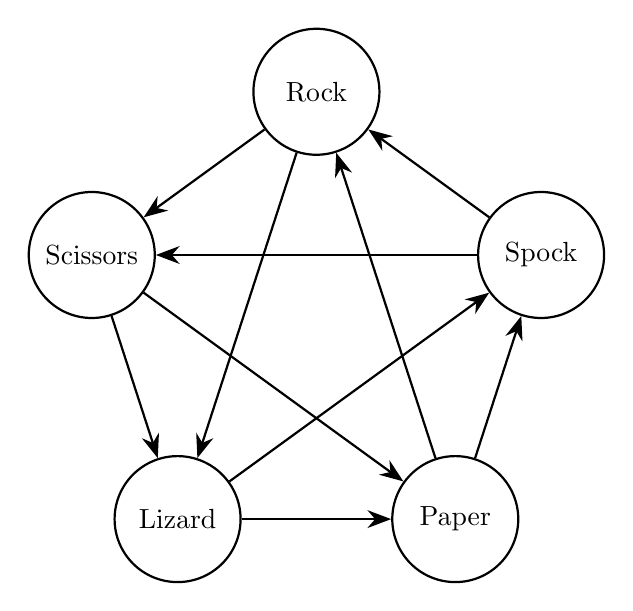
\begin{tikzpicture}[
    thick,
    ->,
    arrow style/.style={-{Stealth[scale=1.3]}},
    object/.style={circle, draw=black, thick, minimum size=1.6cm}
  ]

  % Nodes on a pentagon
  \node[object] (rock)     at (90:3cm)     {Rock};
  \node[object] (spock)    at (18:3cm)     {Spock};
  \node[object] (paper)    at (306:3cm)    {Paper};
  \node[object] (lizard)   at (234:3cm)    {Lizard};
  \node[object] (scissors) at (162:3cm)    {Scissors};

  % Rock beats Scissors and Lizard
  \draw[arrow style] (rock) -- (scissors);
  \draw[arrow style] (rock) -- (lizard);

  % Paper beats Rock and Spock
  \draw[arrow style] (paper) -- (rock);
  \draw[arrow style] (paper) -- (spock);

  % Scissors beats Paper and Lizard
  \draw[arrow style] (scissors) -- (paper);
  \draw[arrow style] (scissors) -- (lizard);

  % Lizard beats Spock and Paper
  \draw[arrow style] (lizard) -- (spock);
  \draw[arrow style] (lizard) -- (paper);

  % Spock beats Scissors and Rock
  \draw[arrow style] (spock) -- (scissors);
  \draw[arrow style] (spock) -- (rock);

\end{tikzpicture}

}

\end{document}